\section{Application of causal discovery to a real system}
\begin{figure}[H]
    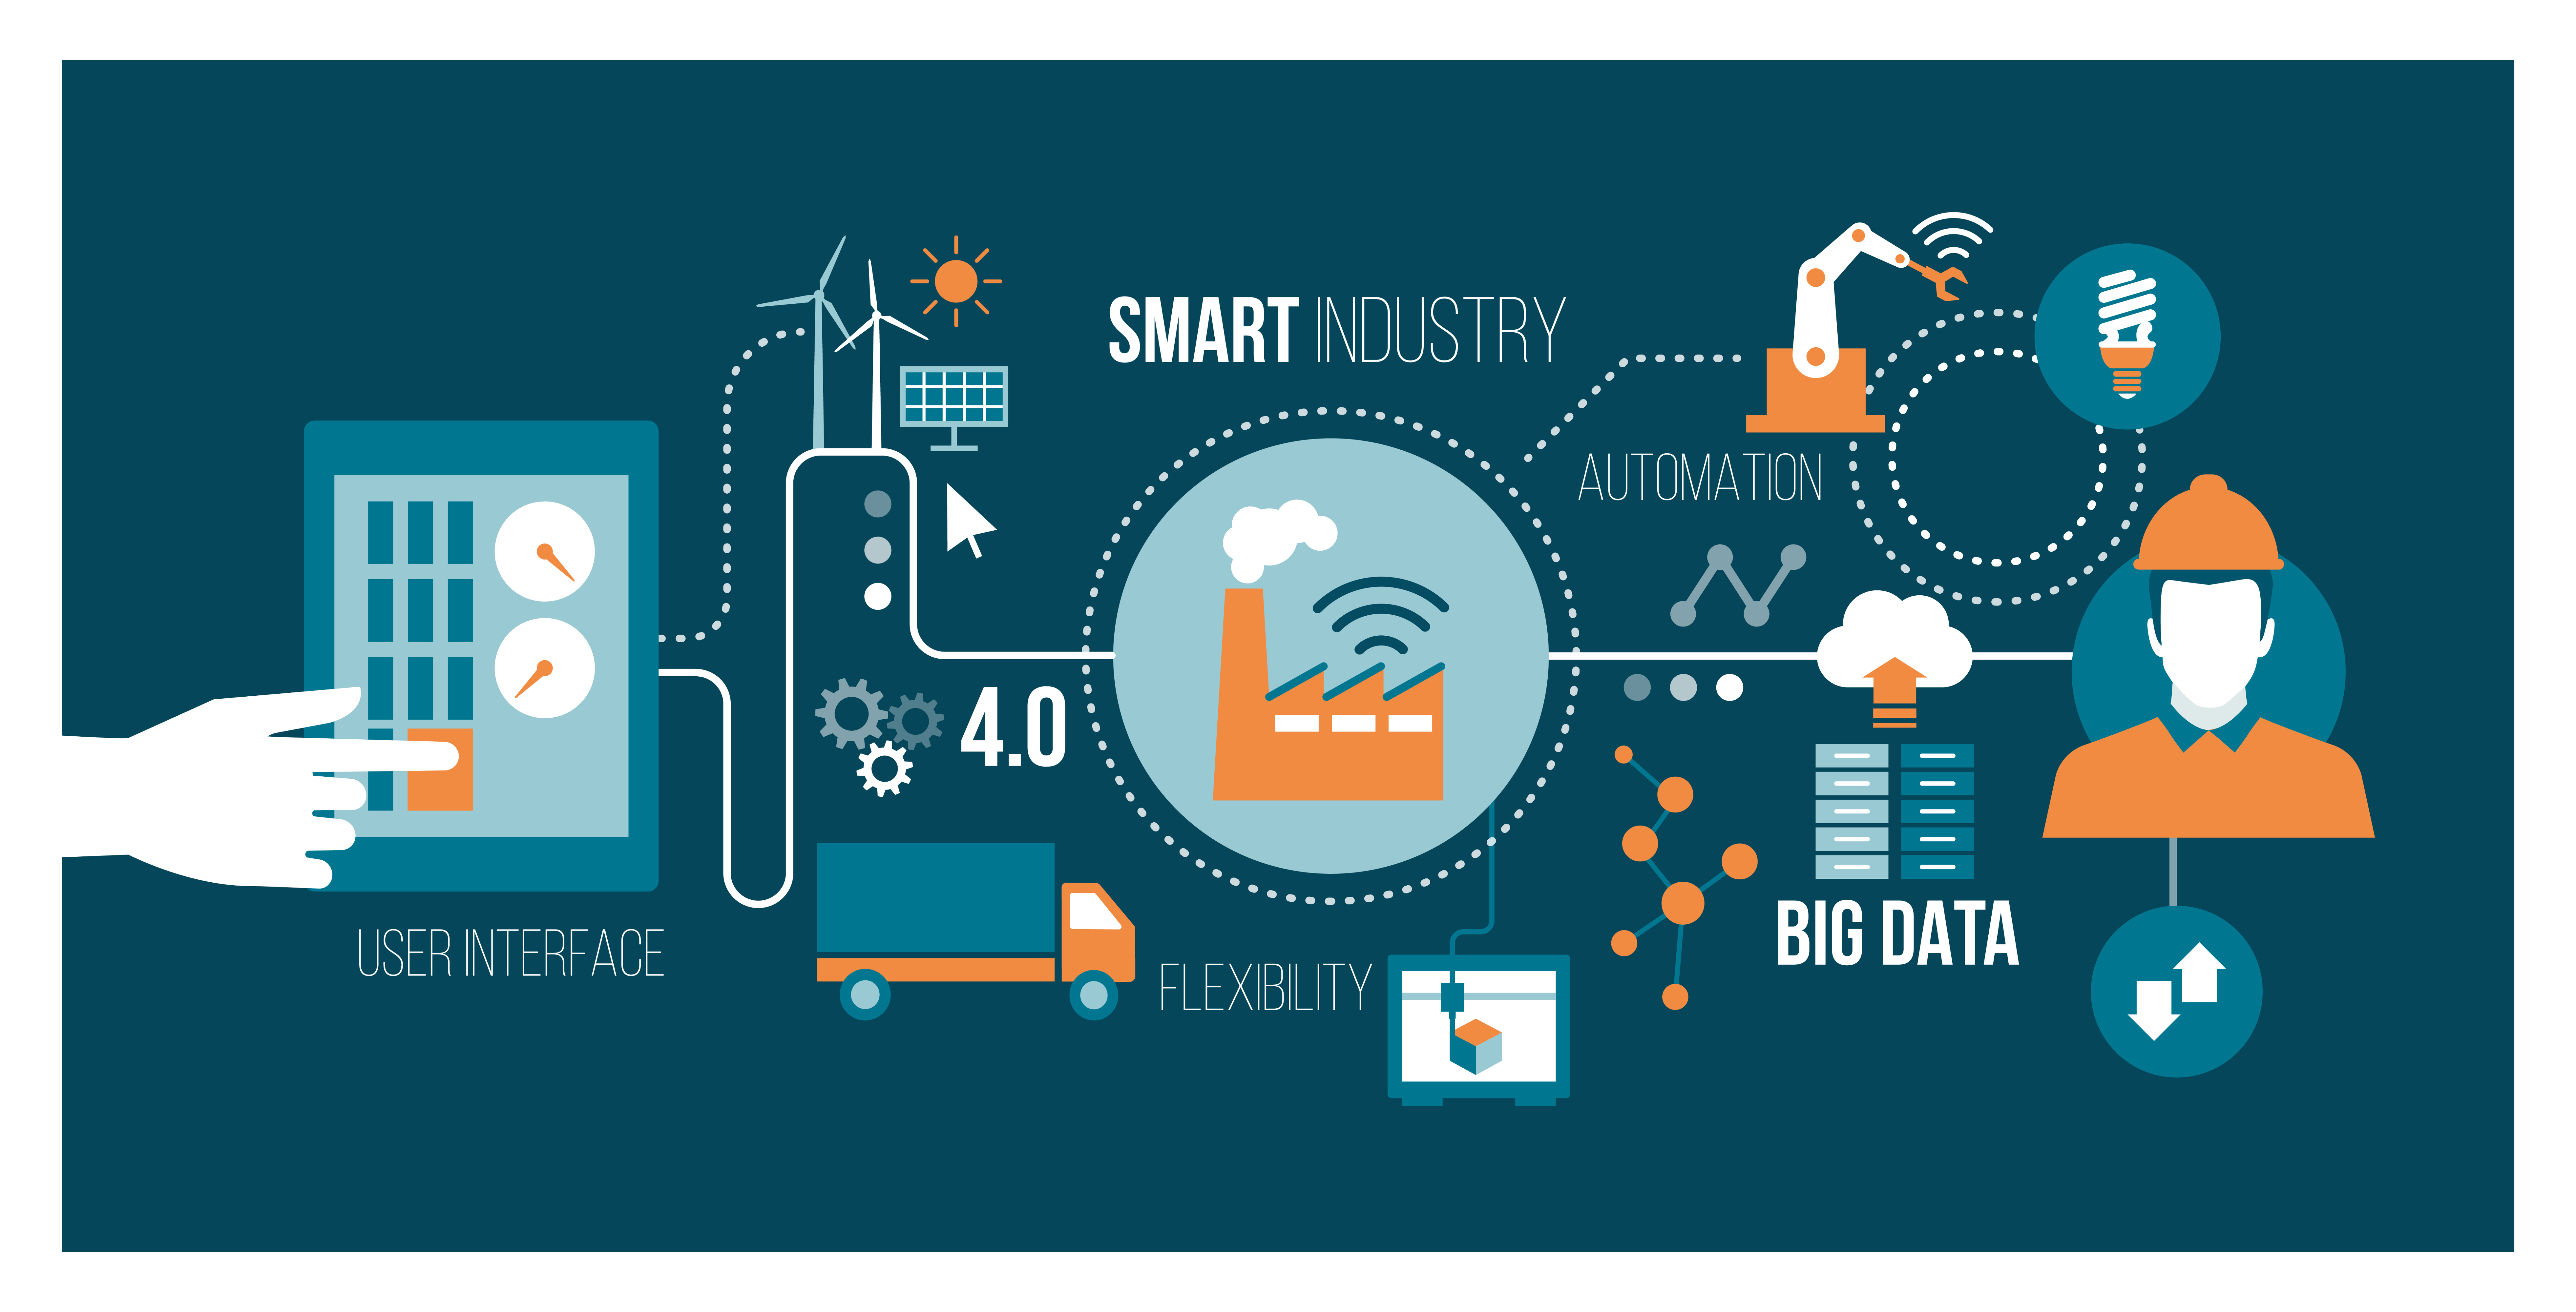
\includegraphics[width=0.7\textwidth]{img/industry4.jpg}
    \centering
    % \caption{'caption'}
\end{figure}
\subsection{Cyber-physical systems(CPS)}
Cyber-physical systems are characterized by a tight interaction between
computational units and physical environment. Those systems have high interaction with humans.
Robots, Industrial Control Systems, Smart Grids and Buildings, Autonomous Cars, $\ldots$ are some examples of CPS.

Those systems pose some Risks (and Challenges) like:
\begin{itemize}
    \item Safety of operators
    \item Cyber attacks
    \item Continual operation
    \item Errors and anomalies are very difficult to detect, due to
    complex physics, architecture and connection of the system.
\end{itemize}

XAI has a great potential for human-machine interaction, predictive maintainance and anomaly
detection, leading to a better exploitation of CPS.

An example of CPS is the SWaT (Secure Water Treatment), a small realistic replication (90
sqm) of a real plant for water filtration and dechlorination in big cities.
It contains 51 sensors/actuators, the dataset contains 11 days of operation.
This example is a well known benchmark for for CPS study and analysis, 
cyber security and assessment of anomaly detection algorithms.
\begin{minipage}[t]{0.4\textwidth}
    \begin{figure}[H]
        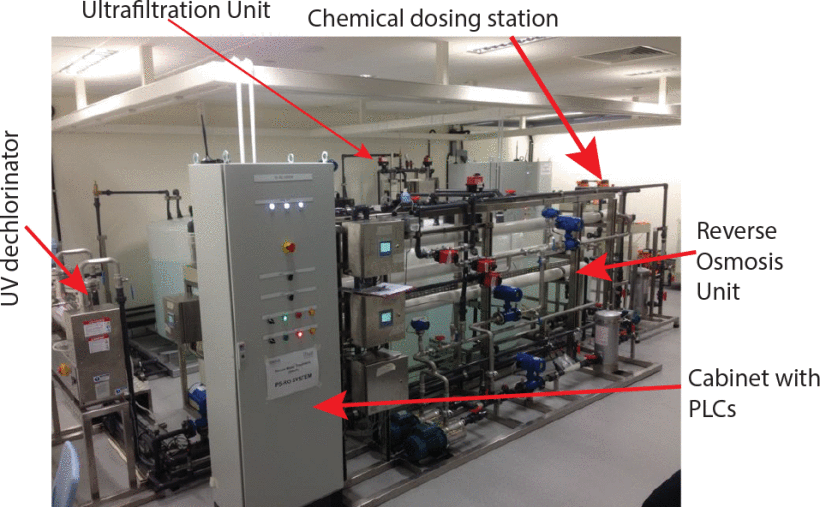
\includegraphics[width=\textwidth]{img/swat.png}
        \centering
    \end{figure}
\end{minipage}
\begin{minipage}[t]{0.5\textwidth}
    \begin{figure}[H]
        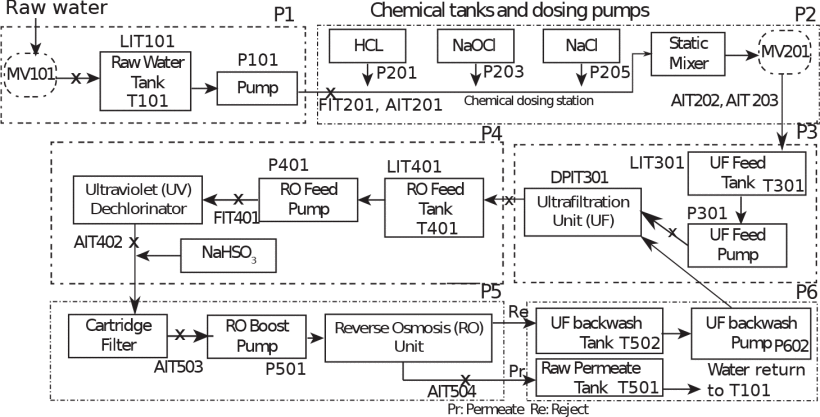
\includegraphics[width=\textwidth]{img/swat_schema.png}
        \centering
    \end{figure}    
\end{minipage}

\subsection{Anomaly Detection}
Physical Systems must ensure continuous operation to do so there is the field of 
Anomaly Detection which goal is to detect anomalies by observing time series representing a system.
There are various approaches:
\begin{itemize}
    \item Online vs Offline
    \item Supervised vs Unsupervised
    \item Single Class vs Open Class
\end{itemize}

\subsubsection*{Unsupervised single class anomaly detection}
\textbf{Online pipeline}
    \begin{itemize}
        \item Collect a dataset of normal behavior
        \item Train a normal model
        \item Use normal model as predictor on anomalous model
        \item Verify discrepancy between prediction and actual readings
    \end{itemize}
Some Algorithms include:
\begin{itemize}
    \item Regression
    \item SVM
    \item PCA
    \item Neural networks
\end{itemize}

\textbf{Offline pipeline}
\begin{itemize}
    \item Collect a dataset of normal behavior
    \item Train a normal model
    \item Train an anomalous model and check the difference with the normal one (or train a model on normal and anomalous data to classify them).
\end{itemize}
\subsubsection*{The role of causal analysis}
Offline anomaly detection identifies normal and anomalous instances of the CPS process, but they don't tell:
\begin{itemize}
    \item What's the origin of the anomaly?
    \item How do multiple anomalies differ?
\end{itemize}
Causal analysis can explain the anomaly.
